\documentclass{jarticle}
\usepackage[dvipdfmx]{graphicx} % Required for inserting images
\usepackage{amsmath}
\usepackage{tikz}
\usepackage{float}
\usepackage{caption}
\usepackage{capt-of}
\usepackage{amsmath}
\usepackage{listings}


\title{設計書}

\begin{document}
\date{}
\maketitle

\section*{設計内容の概要}
\begin{itemize}
    \item ユーザーは、LINEメッセージで目覚ましアラームを「MMDDhhmm」形式で指定する。曜日指定によるルーティン機能にも対応し、アラームの有効・無効を切り替えることも可能。\\
    \item Remo 3 のセンサと外部API（気象庁・天文台API）を利用し、以下の情報を毎日取得：\\
        \begin{enumerate}
            \item 日の出・日没時刻\\
            \item 天気（晴れ・曇り・雨）\\
        \end{enumerate}
    \item 取得情報に基づいて以下の制御を行う：\\
        \begin{enumerate}
            \item 日の出時刻：目覚まし時刻の設定がない場合照明ON\\
            \item 日没1時間前：ユーザーが在宅の場合のみ照明ON\\
            \item 天気による日の出及び起床時に点灯する照明色変化（晴れ＝白、曇り＝青白、雨＝黄）\\
        \end{enumerate}
    \item ユーザーは単純な電気のオンオフ機能や明るさ調整も行うことができる。
\end{itemize}

\section*{システム処理の流れ}
\begin{itemize}
    \item 日次初期化処理（午前0時に実行）\\
        \begin{enumerate}
            \item 日次初期化処理（午前0時に実行）\\
            \item 天気APIから天気を取得 \\
            \item スケジュール登録（Google スプレッドシート）\\
        \end{enumerate}
    \item 目覚まし制御 \\
        \begin{enumerate}
            \item LINEから指定された時刻を受信・解析\\
            \item 指定時刻にアラーム動作（照明ON及びメッセージ通知）\\
            \item 曜日指定時はその曜日にのみ実行 \\
        \end{enumerate}
    \item  天気と照明色の連動\\
        \begin{enumerate}
            \item 天気APIから情報取得\\
            \item 照明の色をプリセットに応じて変更（Remo登録済み赤外線信号で実現）\\
        \end{enumerate}
    \item 日没時の照明点灯\\
          \item 日没時に照明を点灯\\
\end{itemize}

\section*{必要なモジュール（.gsファイル）}

\begin{enumerate}
  \item \textbf{reciever.gs}
  \begin{itemize}
    \item LINE Webhook の受信
    \item ユーザーからのコマンド（MMDDhhmm形式など）の解析
    \item スケジュールデータの登録・管理
  \end{itemize}

  \item \textbf{checker.gs}
  \begin{itemize}
    \item 目覚ましスケジュールの登録と実行
    \item 日の出・日没イベントの管理
    \item 曜日指定やスヌーズ対応など
    \item 照明のON・OFFの対応
  \end{itemize}

  \item \textbf{deleter.gs}
  \begin{itemize}
    \item 週アラーム機能のリセット
  \end{itemize}

  \item \textbf{weather.gs}
  \begin{itemize}
    \item 気象庁APIやOpenWeatherMapからの天気情報取得
    \item 天気データの解析（晴れ・曇り・雨の判定）
  \end{itemize}

  \item \textbf{getSunRise.gs}
  \begin{itemize}
    \item APIで日の出時刻の取得
  \end{itemize}

  \item \textbf{getSunSet.gs}
  \begin{itemize}
    \item APIで日の入時刻の取得
  \end{itemize}

  \item \textbf{alarm\_controller.gs, alarm.gs}
  \begin{itemize}
    \item アラーム時の赤外線信号の送信
    \item スヌーズ機能の実装
  \end{itemize}

  \item \textbf{controllerフォルダ以下のgsファイル}\\
  各照明によって指示が異なるため、複数用意している。
  \begin{itemize}
    \item 天気や照度、日の出・日没時間に応じた照明制御
    \item 照明の色や明るさの変更処理
  \end{itemize}
\end{enumerate}

\section*{クラス図}
以下にクラス図を示す

\begin{figure}[H]  % [H] はその場所に固定
  \begin{center}
    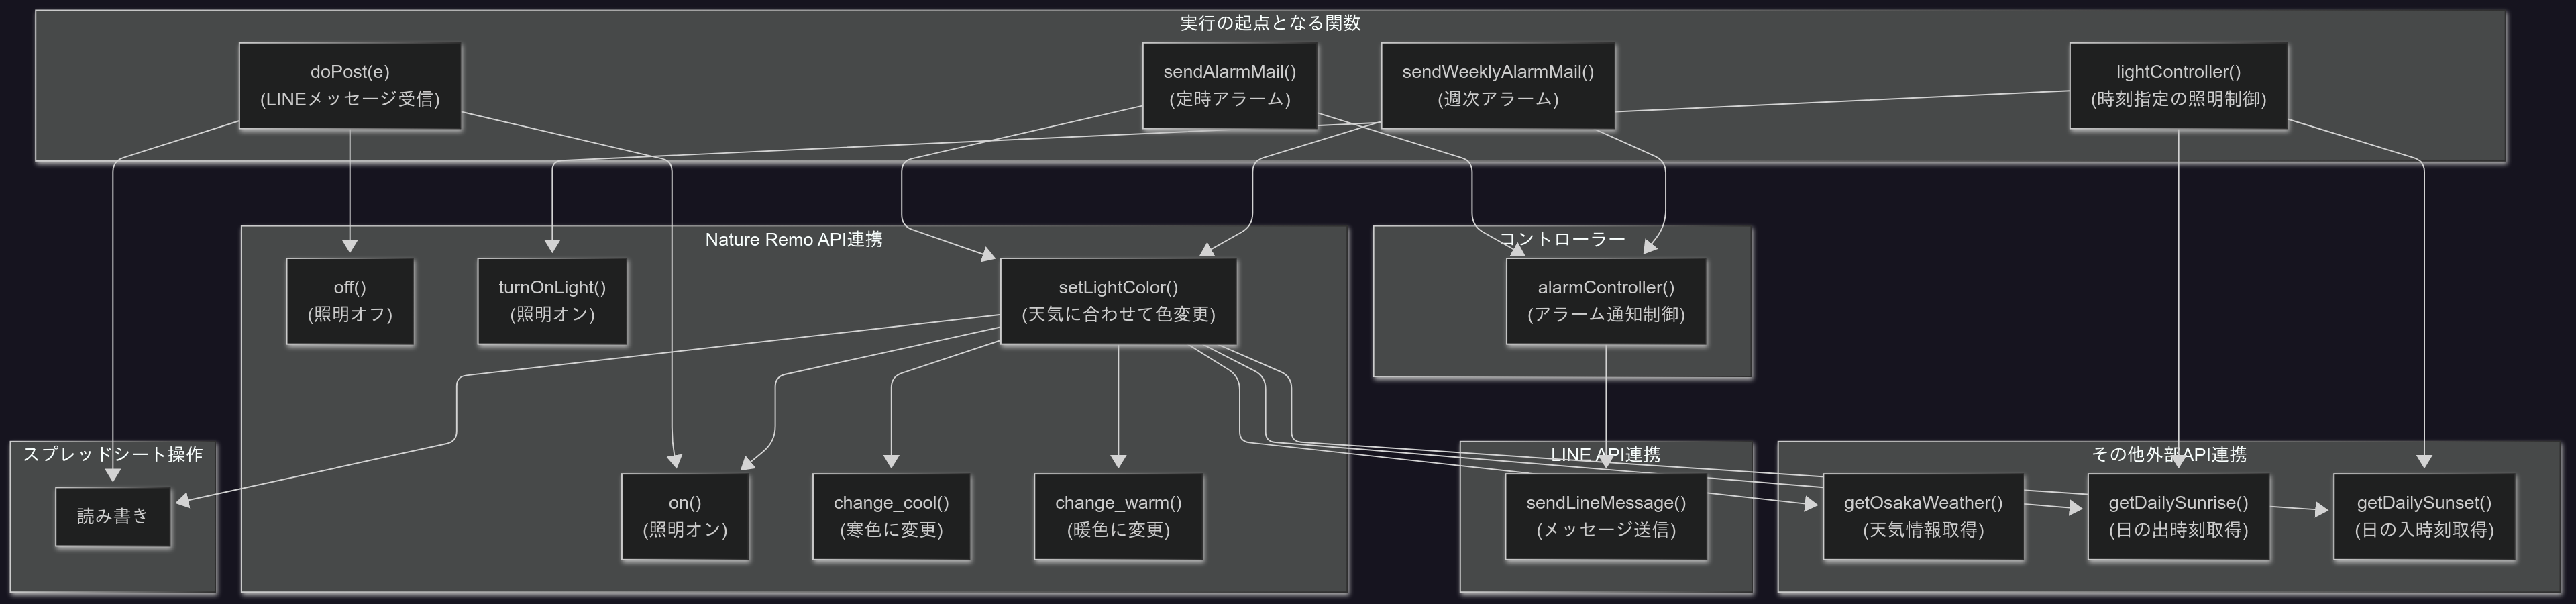
\includegraphics[scale = 0.11]{./fig/class.eps}
    \caption{クラス図}
    \label{fig:class}
  \end{center}
\end{figure}

\section*{シーケンス図}
以下にシーケンス図を示す

\begin{figure}[H]  % [H] はその場所に固定
  \begin{center}
    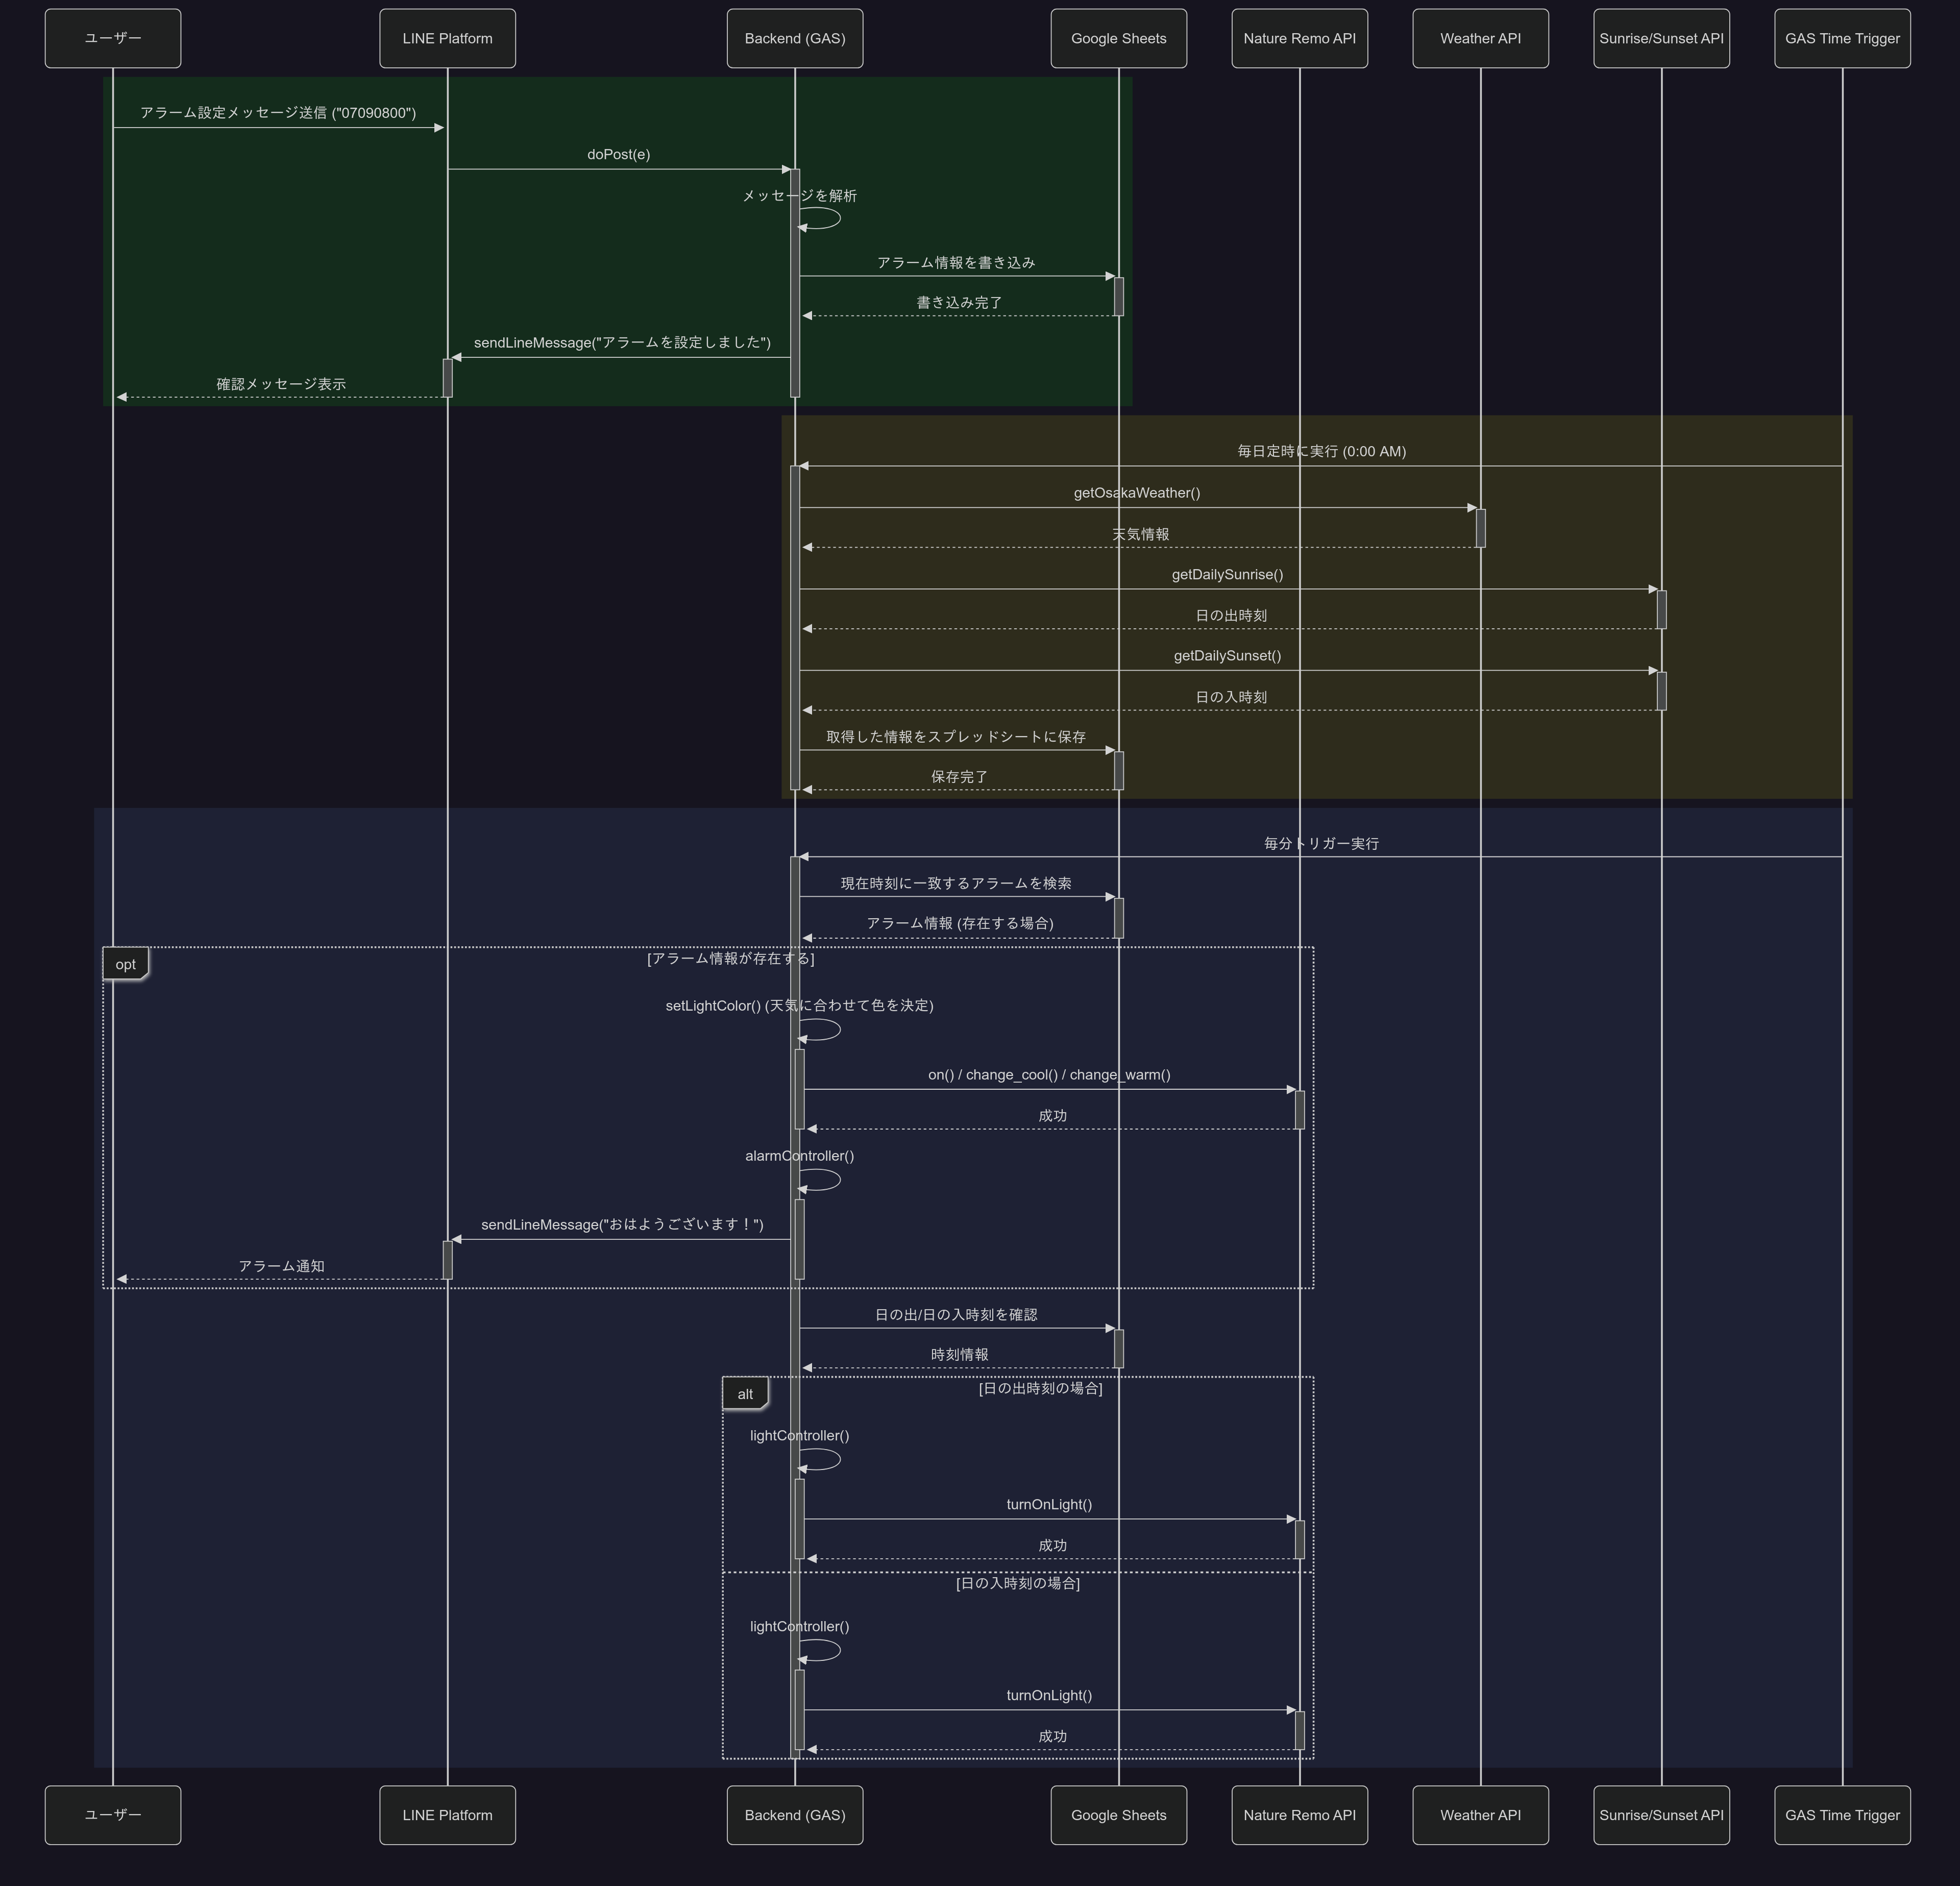
\includegraphics[scale = 0.11]{./fig/seq.eps}
    \caption{クラス図}
    \label{fig:seq}
  \end{center}
\end{figure}


\end{document}